\documentclass[11pt]{beamer}
\usepackage[utf8]{inputenc}
\usepackage[spanish]{babel}
\usepackage{amsmath}
\usepackage{amsfonts}
\usepackage{amssymb}
\usepackage{graphicx}
\usepackage{caption}
\usepackage{subcaption}
\usepackage{lipsum}
\usepackage{ragged2e}
\usepackage{hyperref}
\usepackage{float}
\usepackage{url}
\usepackage{multicol}
\usetheme{Madrid}
\newcommand{\celda}[1]{
	\begin{minipage}{2.5cm}
		\vspace{5mm}
		#1
		\vspace{5mm}
	\end{minipage}
}
\newtheorem{teorema}{Teorema}[section]
\newtheorem{proposicion}{Proposición}[section]
\newtheorem{definicion}{Definición}[section]
\newtheorem{nota}{Nota}[section]
\newtheorem{corolario}{Corolario}[section]

\author[Christian Paredes A.]{\footnotesize Christian Paredes Aguilera \\ \vspace{4mm} En colaboración con:\\ \vspace{1mm} Gabriel Rosario Roselló  \\ Jorge Valero \\\vspace{4mm} {\color{blue} XI Congreso InvestMat}}
\title [XI Congreso InvestMat] {Coherencia wavelet, una herramienta para el análisis dinámico entre series temporales.}
\date{10 Enero 2024} 

\logo{
    
\includegraphics[width=1cm,height=1cm,keepaspectratio]{logouv.jpg}
    
\includegraphics[width=1cm,height=1cm,keepaspectratio]{upvlogo.jpg}
    }



%\AtBeginSection[]
%{
%	\begin{frame}<beamer>{Índice}
%		\tableofcontents[currentsection,currentsubsection]
%	\end{frame}
%}


\begin{document}
\begin{frame}
		\maketitle
	\end{frame}

	\begin{frame}{\footnotesize Coherencia wavelet, una herramienta para el análisis dinámico entre series temporales.}
		\tableofcontents
	\end{frame}
	
\section{Introducción}
	

    % ------------------------ INTRODUCCIÓN ------------------------
    \begin{frame}{Introducción}

	Existen diversas técnicas, para analizar completamente dos variables a lo largo del tiempo:
	\vspace{5mm}
	\begin{itemize}
	    \item Coeficiente de correlación de Pearson $\rightarrow$ \textbf{Correlación}.
	    \item Series de Fourier $\rightarrow$ \textbf{Frecuencia}.
	    \item Causalidad de Granger $\rightarrow$ \textbf{Causalidad}.
	\end{itemize}
    \end{frame}

    %PÁGINA 4
    \begin{frame}{Introducción}

	\begin{center}
	    ¿Existe otra técnica que sea capaz de análisis conjuntamente la Correlación, la Frecuencia, la Causalidad y más?
	\end{center}

	\begin{center}
	    SI!!!
	\end{center}

	\begin{center}
	    WAVELETS: Coherencia wavelet y diferencia de fase.
	\end{center}

    \end{frame}

    %PÁGINA 5
    \begin{frame}{Introducción}{Ventajas de usar wavelets}
	Ventajas de usar wavelets en series de tiempo:
	\vspace{5mm}
	\begin{itemize}	
	    \item Resolución en tiempo y frecuencia.
	    \item Análisis multiescala.
	    \item Manejo de datos no estacionarios.
	\end{itemize}

    \end{frame}

    %PÁGINA 6
    \begin{frame}{Introducción}{Definición de coherencia wavelet}
	Cuando hablamos de coherencia wavelet, nos referimos a una relación dinámica.

	\begin{definicion}
	    La coherencia wavelet entre dos series de tiempo $x(t)$ e $y(t)$ es una función de tiempo y escala definida por:
	    \begin{equation}
		R^{2}_{xy}(\tau,s)=\frac{\left|S\left(s^{-1}W_{xy;\psi(\tau,s)}\right)\right|^2}{S\left(s^{-1}\left|W_{x;\psi}(\tau,s)\right|^2\right)S\left(s^{-1}\left|W_{y;\psi}(\tau,s)\right|^2\right)}
	    \end{equation}
	\end{definicion}

    \end{frame}

    %PAGINA 7
    \begin{frame}{Introducción}{Ejemplo}
	Demos un ejemplo:

	\begin{center}
	    Café vs. $\pi$zzas
	\end{center}
	%2 columnas 
	\begin{multicols}{2}
	     \begin{figure}
		 
\includegraphics[scale=0.12]{cafePizza.jpeg}
		 %\caption{Morlet Wavelet $\psi=e^{-t^2/2}cos(5t)$}
		 %\label{fig:enter-label}
	     \end{figure}
	     $\frac{\left|S\left(s^{-1}W_{xy;\psi(\tau,s)}\right)\right|^2}{S\left(s^{-1}\left|W_{x;\psi}(\tau,s)\right|^2\right)S\left(s^{-1}\left|W_{y;\psi}(\tau,s)\right|^2\right)}$
	     \vspace{5mm}
	    En pocas palabras la coherencia wavelet es el grado con el que \textbf{correlacionan} dos series de temporales en función del \textbf{tiempo} y la \textbf{frecuencia}.
	\end{multicols}

    \end{frame}

	
    %PAGINA 8
    % ------------------------ OBJETIVO ------------------------
    \begin{frame}{Objetivo}

	Ahora, para hablar de \textbf{causalidad}, necesitamos definir \textbf{diferencia de fase}. Que será el objetivo de esta presentación, seguido de detallar los \textbf{datos} analizados y presentar \textbf{resultados} empíricos.

    \end{frame}


\section{Construcción}

    %PAGINA 9
    \begin{frame}{Construcción}{Transformada Wavelet Cruzada}

    La \textbf{transformada de wavelet cruzada} de dos series de tiempo $x(t)$ y $y(t)$ se define como:

    \begin{definicion}
    \begin{equation}
    W_{xy;\psi}(\tau, s) = W_{x;\psi}(\tau, s)W_{y;\psi^*}(\tau, s)
    \end{equation}
    \end{definicion}

    \end{frame}

    %PAGINA 10
    \begin{frame}{Construcción}{Diferencia de Fase}

    La \textbf{diferencia de fase} entre $x(t)$ y $y(t)$ se define como:

    \begin{definicion}
    \begin{equation}
	\phi_{xy}=\tan^{-1} \left(\frac{\mathfrak{J}\left\{S\left(s^{-1}W_{xy;\psi}(\tau,s)\right)\right\}}{\mathfrak{R} \left\{S\left(s^{-1}W_{xy;\psi}(\tau,s)\right)\right\}}\right),\quad \mbox{con}\quad \varphi_{xy}\in[-\pi,\pi].
    \end{equation}
    \end{definicion}

    Donde $\mathfrak{J}$ y $\mathfrak{R}$ son las partes imaginarias y reales de la transformada de wavelet cruzada suavizada, respectivamente.

    \end{frame}

    %PAGINA 11
    \begin{frame}{Construcción}{Retraso de Tiempo Instantáneo}

    Podemos convertir la diferencia de fase en el \textbf{retraso de tiempo instantáneo} entre $x(t)$ y $y(t)$ de la siguiente manera:

    \begin{equation}
	(\Delta t)_{xy}=\frac{\phi_{xy}}{2\pi f},
    \end{equation}

    Donde $2\pi f$ es la frecuencia angular con respecto a la escala de tiempo $s$, y la frecuencia de Fourier usual $f$ se da por:

    \begin{equation}
	f = \frac{\omega_\psi}{2\pi s},
    \end{equation}

    Por lo tanto, el retraso de tiempo $(\Delta t)_{xy}$ se da finalmente por:

    \begin{equation}
	(\Delta t)_{xy}=\frac{\varphi_{xy}\cdot s}{2\pi},
    \end{equation}

    \end{frame}

    %PAGINA 12
    \begin{frame}{Construcción}{Interpretación de las Flechas}

    Las diferencias de fase se representan como flechas en los gráficos de coherencia de wavelet. La dirección de las flechas tiene los siguientes significados:

    \begin{itemize}
	\item \textbf{Flechas apuntando a la derecha:} $x(t)$ y $y(t)$ están en fase (o relacionadas positivamente).
	\item \textbf{Flechas apuntando a la izquierda:} $x(t)$ y $y(t)$ están fuera de fase (o relacionadas negativamente).
	\item \textbf{Flechas apuntando hacia arriba:} $x(t)$ adelanta a $y(t)$ en un cuarto de la escala correspondiente o se retrasa detrás de $y(t)$ en tres cuartos de la escala correspondiente.
	\item \textbf{Flechas apuntando en otras direcciones:} indican retrasos o adelantos entre $x(t)$ y $y(t)$.
    \end{itemize}

    Las diferencias de fase también pueden sugerir causalidad entre $x(t)$ y $y(t)$.

    \end{frame}

    %PAGINA 13
    \begin{frame}{Construcción}{Ejemplo}
	     \begin{figure}
		 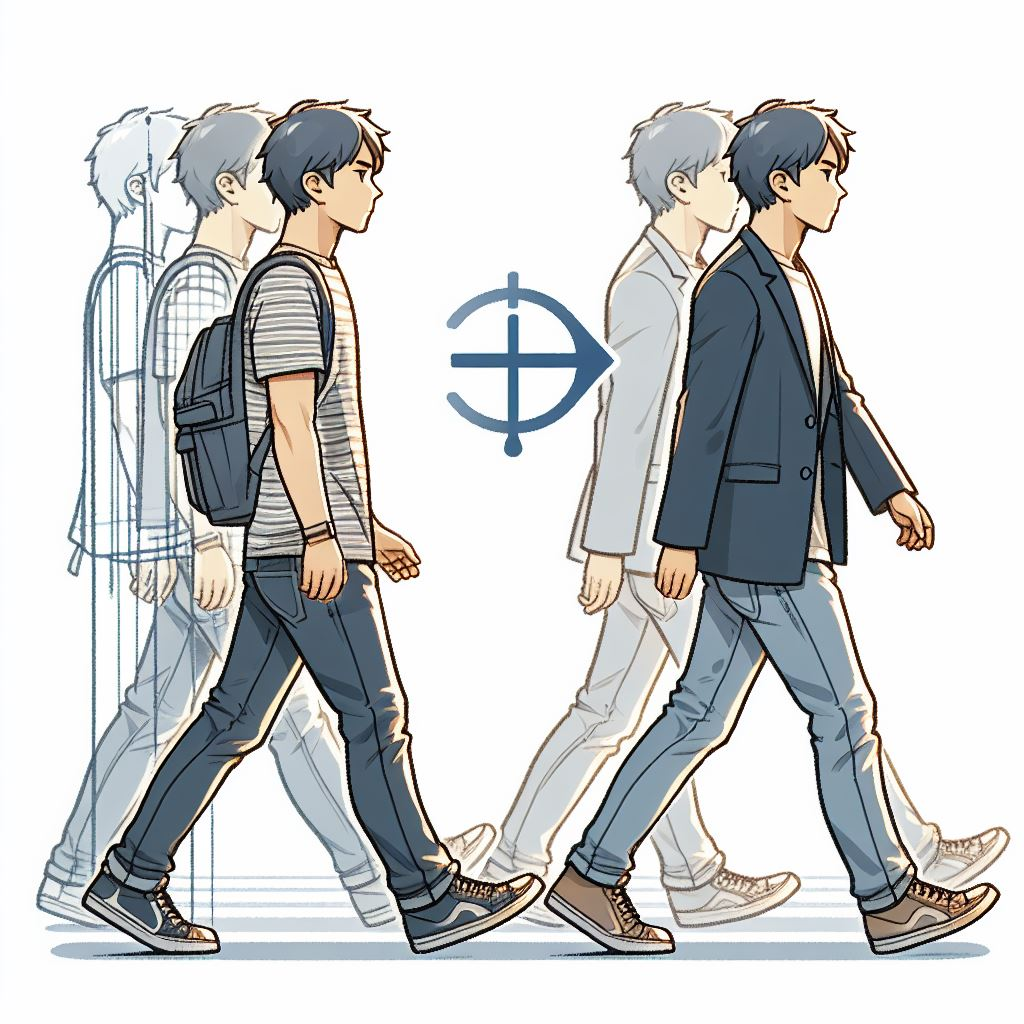
\includegraphics[scale=0.18]{ejemPasos.jpeg}
	     \end{figure}
    \end{frame}

    

\section{Resultados de datos empíricos}

    %PAGINA 13
    \begin{frame}{Resultados de datos empíricos}{Descripción de datos}
	Utilizamos datos mensuales de la Unión Europea a partir de enero de 1997 hasta octubre de 2023. Extraídos del Banco Central de Europa, de las variables:
	\begin{multicols}{2}
	     \begin{figure}
		 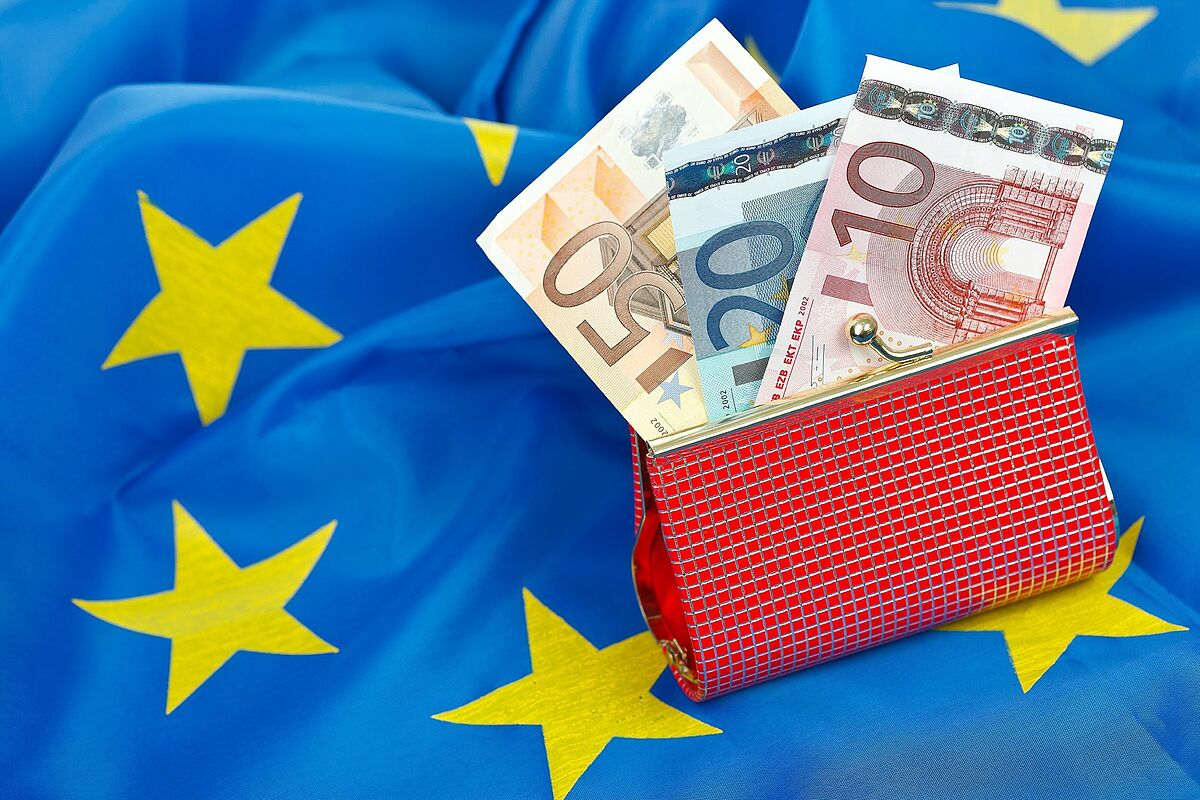
\includegraphics[scale=0.18]{euroZona.jpg}
		 %\caption{Morlet Wavelet $\psi=e^{-t^2/2}cos(5t)$}
		 %\label{fig:enter-label}
	     \end{figure}
	\begin{itemize}
	    \item \textbf{Crecimiento de dinero (HIPC)}.
	\item \textbf{Inflación (M1)}.
	\end{itemize}
	\end{multicols}
    \end{frame}

     %PAGINA 14
    \begin{frame}{Resultados de datos empíricos}{Gráficos de series de tiempo}
	\begin{multicols}{2}
	    \begin{figure}[H]
		\centering
		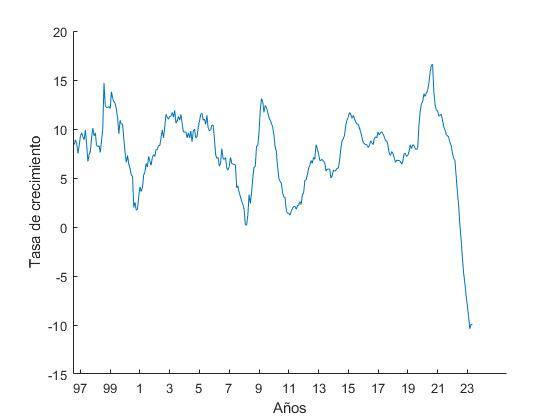
\includegraphics[scale=0.32]{M1s.jpg}
		\caption{\tiny Señal relativa al agregado monetario M1. Elaboración propia.}
		\label{fig:M1}
	    \end{figure}

	    \begin{figure}[H]
		\centering
		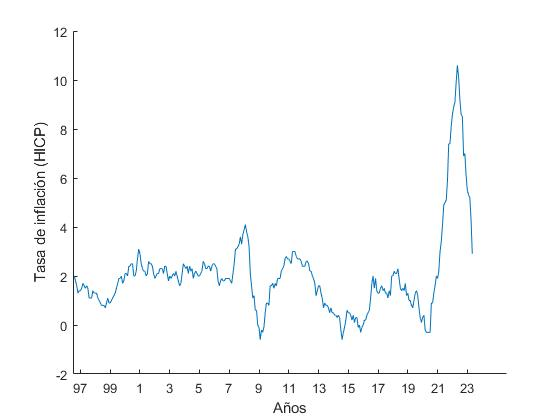
\includegraphics[scale=0.32]{infs.jpg}
		\caption{\tiny Señal relativa al HICP (Harmonised Index of Consumer Prices). Elaboración propia.}
		\label{fig:inf}
	    \end{figure}
	\end{multicols}
    \end{frame}

    %PAGINA 15
    \begin{frame}{Resultados de datos empíricos}{Series de Fourier}
	\begin{multicols}{2}
	    \begin{figure}[H]
		\centering
		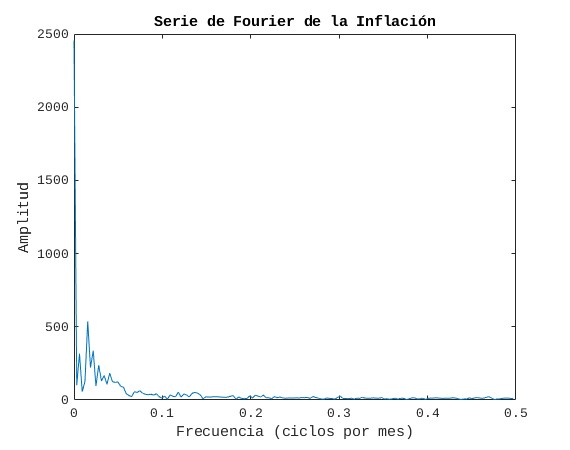
\includegraphics[scale=0.32]{fourierInflacion.jpg}
		\caption{\tiny Transformada de Fourier de agregado monetario M1. Elaboración propia.}
		\label{fig:M1}
	    \end{figure}

	    \begin{figure}[H]
		\centering
		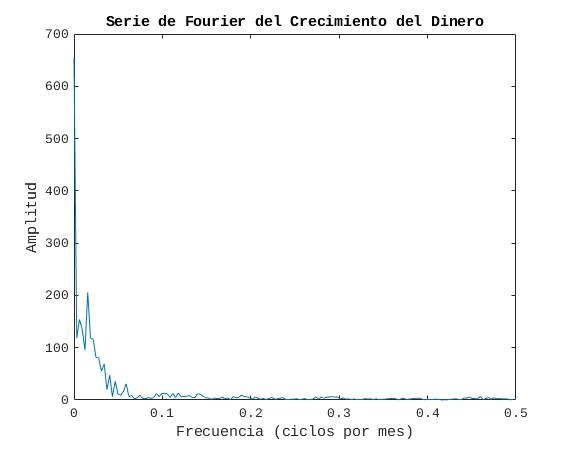
\includegraphics[scale=0.32]{fourierDinero.jpg}
		\caption{\tiny Transformada de Fourier de HICP (Harmonised Index of Consumer Prices). Elaboración propia.}
		\label{fig:inf}
	    \end{figure}
	\end{multicols}
    \end{frame}

    %PAGINA 16
    \begin{frame}{Resultados de datos empíricos}{Causalidad de Granger}
	\begin{table}[h]
	    \centering
	    \begin{tabular}{|l|l|l|}
		\hline
		H0 & Decision & Distribution \\ \hline
		Exclude lagged Y1 in Y2 equation & Cannot reject H0 & Chi2(10) \\ \hline
	    \end{tabular}

	    \begin{tabular}{|l|l|}
		\hline
		Statistic & PValue \\ \hline
		14.14 & 0.16671 \\ \hline
	    \end{tabular}

	    \begin{tabular}{|l|}
		\hline
		CriticalValue \\ \hline
		18.307 \\ \hline
	    \end{tabular}
	    \caption{\tiny Resultados de la prueba de causalidad de Granger. Elaboración propia.}
	    \label{tab:granger}
	\end{table}

    \end{frame}

    %PAGINA 17
    \begin{frame}{Resultados de datos empíricos}{Coherencia Wavelet y diferencia de fase}
	    \begin{figure}[H]
		\centering
		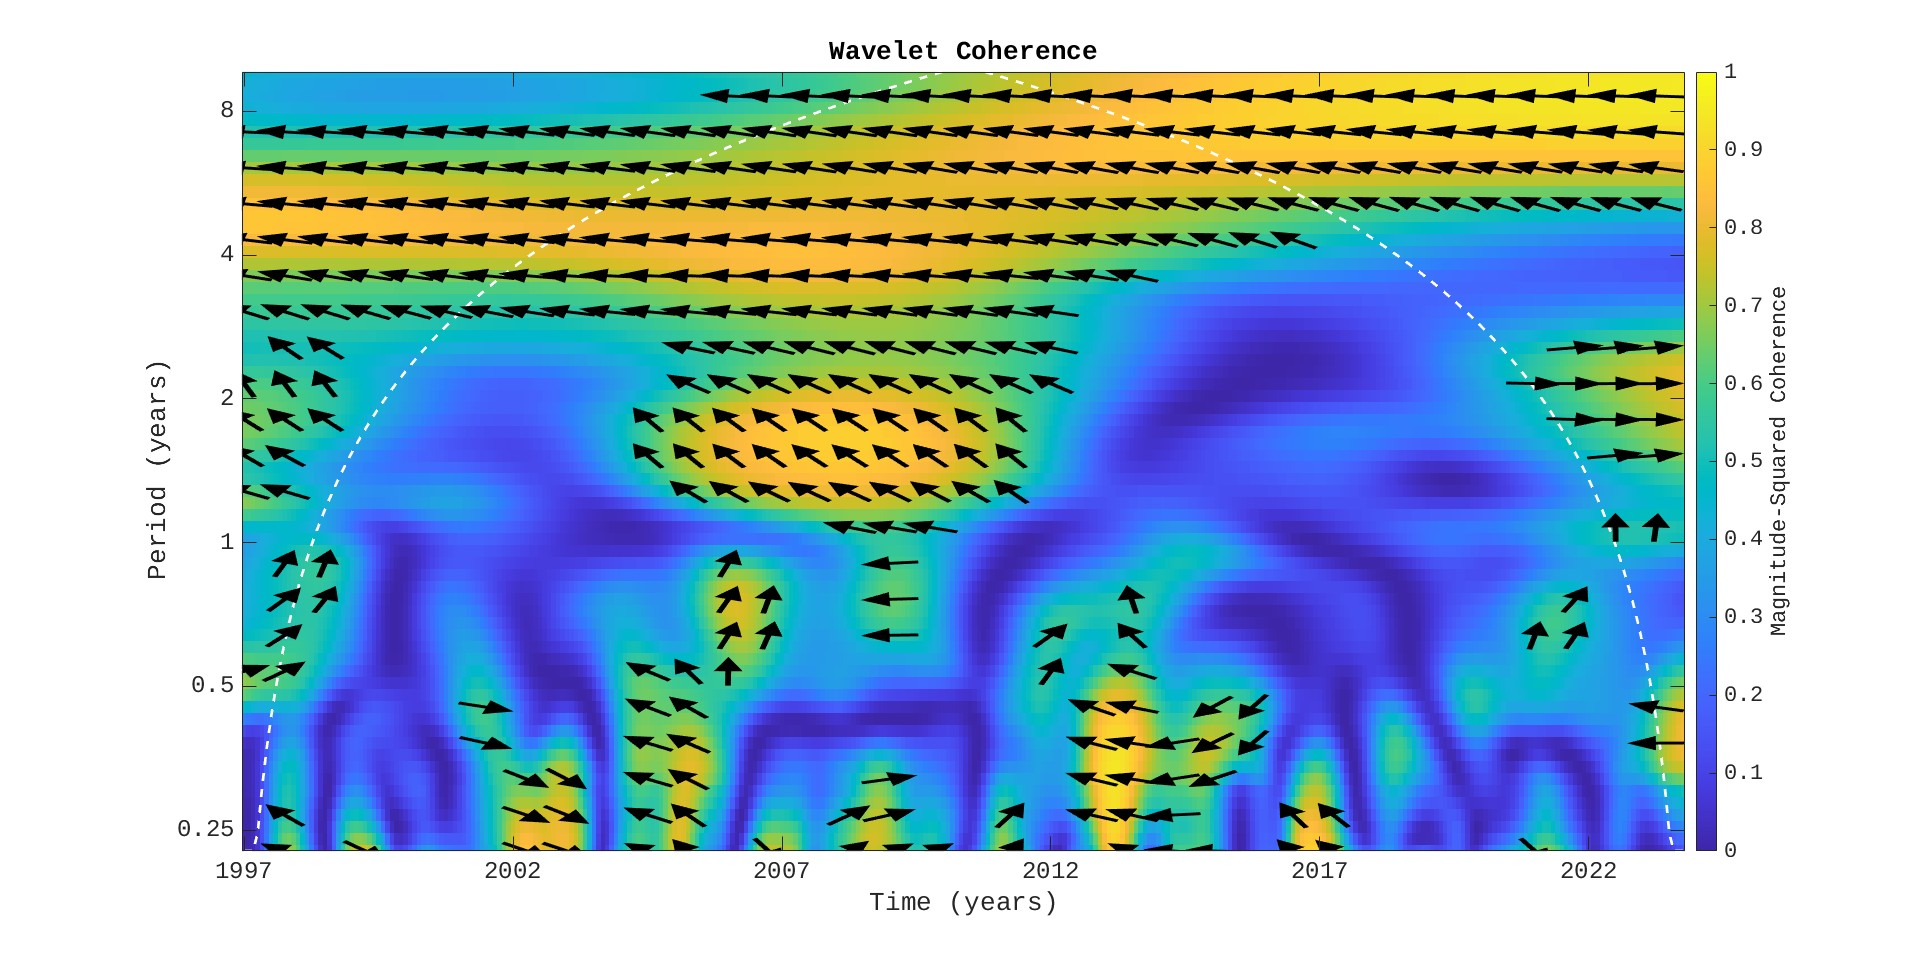
\includegraphics[scale=0.175]{coherenciaFase.jpg}
		\caption{\tiny Transformada de Fourier de HICP (Harmonised Index of Consumer Prices). Elaboración propia.}
		\label{fig:inf}
	    \end{figure}
    \end{frame}


    \section{Conclusión}
    %PAGINA 18
    \begin{frame}{Conclusión}
	La \textbf{Coherencia Wavelet} y su complemento la Diferencia de Fase son técnicas poderosas para el análisis de series de tiempo. Permiten analizar la correlación en tiempo y frecuencia, así como la relación causal entre dos variables. A diferencia de otras técnicas como la correlación de Pearson, la transformada de Fourier y la causalidad de Granger, estas proporcionan una visión más dinámica de las relaciones entre las series de tiempo. Son especialmente útiles para manejar datos no estacionarios y proporcionar una visión detallada de cómo las relaciones entre las variables cambian con el tiempo y a diferentes frecuencias.
    \end{frame}

    \begin{frame}{Fin}
    \begin{center}
        {\huge Fin}
        
        \vspace{5mm}
        {\large ¡Muchas gracias por vuestra atención!}
    \end{center}
    \end{frame}

    \section{Bibliografía}
    \begin{frame}{Bibliografía}
        \begin{thebibliography}{99}


    \bibitem{POR} 
    \textsc{Aguiar-Conraria, L., Azevedo, N. \& Soares, M.J.}, \textit{Using wavelets to decompose the time-frequency effects of monetary policy}, Physica A: Statistical Mechanics and its Applications {\bf 387}  (2008), pp., 2863-2878.  
    
    \bibitem{MGI2015} 
    \textsc{Jiang, C., Chang, T., Li XL.}, \textit{Money growth and inflation in China: New evidence from a wavelet analysis}, International Review of Economics \& Finance {\bf 35}, (2015), pp. 249-261. 

    \bibitem{PGWA} 
    \textsc{Torrence C. \& Compo, G.}, \textit{A Practical Guide to wavelet analysis}, Bulletin of the American Meteorological Society {\bf 79}  (1998), pp., 61-78.  

    \bibitem{BCE}
    \href{https://data.ecb.europa.eu/data}{European Central Bank}

\end{thebibliography}
    \end{frame}
	
\end{document}
